% New independently generated TikZ diagram (original external asset was not included).
% Exact model: x^2/4-y^2/5=1; A1=(-2,0), A2=(2,0), P1=(3,5/2), P2=(-3,-5/2).
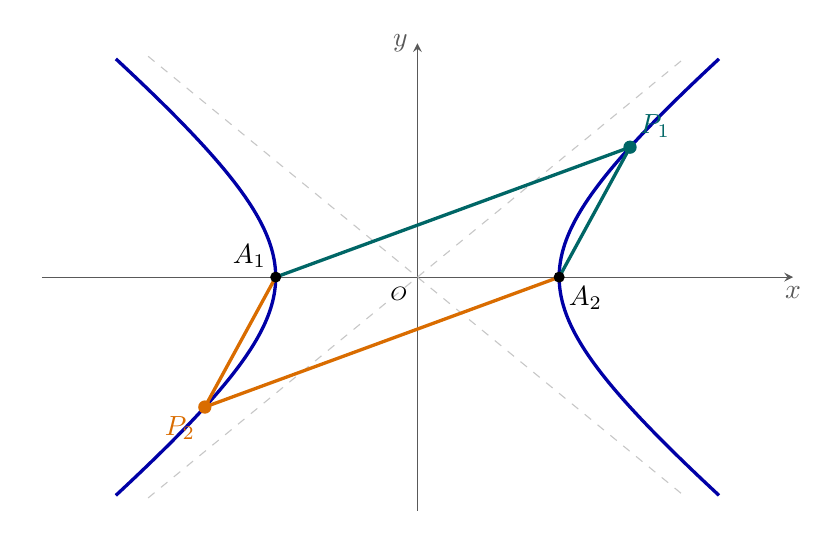
\begin{tikzpicture}[x=0.9cm,y=0.66cm,>=stealth]
 \clip (-5.5,-4.7) rectangle (5.5,4.8);
 \draw[->,black!65,thin] (-5.3,0)--(5.3,0) node[below] {$x$};
 \draw[->,black!65,thin] (0,-4.5)--(0,4.5) node[left] {$y$};
 \draw[dashed,black!22] (-3.8,-4.249)--(3.8,4.249);
 \draw[dashed,black!22] (-3.8,4.249)--(3.8,-4.249);
 \draw[very thick,blue!65!black,domain=-4.2:4.2,samples=80,smooth,variable=\t]
   plot ({sqrt(4+(4/5)*\t*\t)},{\t});
 \draw[very thick,blue!65!black,domain=-4.2:4.2,samples=80,smooth,variable=\t]
   plot ({-sqrt(4+(4/5)*\t*\t)},{\t});
 \coordinate (A1) at (-2,0);
 \coordinate (A2) at (2,0);
 \coordinate (P1) at (3,2.5);
 \coordinate (P2) at (-3,-2.5);
 \draw[very thick,teal!80!black] (A1)--(P1) (A2)--(P1);
 \draw[very thick,orange!85!black] (A1)--(P2) (A2)--(P2);
 \fill (A1) circle (2pt) node[above left] {$A_1$};
 \fill (A2) circle (2pt) node[below right] {$A_2$};
 \fill[teal!80!black] (P1) circle (2.4pt) node[above right] {$P_1$};
 \fill[orange!85!black] (P2) circle (2.4pt) node[below left] {$P_2$};
 \node[below left,font=\scriptsize] at (0,0) {$O$};
\end{tikzpicture}
